\documentclass[10pt]{article}
\usepackage[margin=0.82in]{geometry}
\usepackage{booktabs,amsmath,graphicx,hyperref,array,microtype,xcolor}
\usepackage[T1]{fontenc}
\microtypesetup{expansion=false}
\newcommand{\pra}{\textsc{PRA}}
\newcommand{\air}{\textsc{AirLLM}}
\newcommand{\evidence}[1]{\textcolor{black!65}{\textsc{#1}}}
\title{Progressive Retrieval Attention with AirLLM:\\
Independent Weight and Semantic-Context Streaming}
\author{Jorge Sim\~ao}
\date{August 2026}

\begin{document}
\maketitle

\begin{abstract}
AirLLM makes models larger than accelerator memory executable by loading one
decoder layer, or selected experts, immediately before use and releasing its
weights afterward. Progressive Retrieval Attention (PRA) addresses a different
state variable: it routes over persistent context and materializes only selected
native key/value (K/V) detail. We ask whether these two forms of virtualization
compose without conflating model-weight and semantic-memory policy. We audit
AirLLM 3.3.0 at commit \texttt{3099999}, implement a capability-gated runtime
provider, reuse the existing Hugging Face PRA attention path, and introduce a
layer-local lifecycle adapter with HOT, layer-streamed, and hybrid PRA residency.
On Apple M5, AirLLM's separate MLX path executes TinyLlama-1.1B from 2.20-GB
layer shards. Reducing a 653-token prompt to 38 selected tokens preserved the
12-token answer prefix, but throughput remained about 0.13 token/s because
weight streaming dominated. In a 119-condition controlled lifecycle study,
layer-streaming reduced balanced-profile PRA peak residency from 0.50 to
0.125 MiB; independent prefetch was faster than sharing AirLLM's one-worker
weight executor. On a 4-GiB GTX 950M, injected-but-disabled PRA preserved the
exact AirLLM output, and native PRA encoded and consumed a 15-token reference
through four layers. Native decode was 10.6\% slower than selected-text E0, so
this establishes mechanism correctness rather than a speed advantage. A
selector-frozen three-example natural-QA follow-up materialized 384 native
tokens while removing 92.9--95.8\% of E0's visible selected-text prompt. Its
cold and warm E2/E0 completion ratios were 0.969--1.016, but both paths scored
zero task F1 and none of nine paired completions matched exactly. The run is
therefore transport and memory evidence, not semantic parity. The
evidence supports independent policy and exposes
the central systems tradeoff: eliminating context residency is valuable only
when its transfers do not deepen the weight-I/O bottleneck.
\end{abstract}

\section{Qualification Snapshot}
\textbf{Engine question.} Can AirLLM virtualize model weights while PRA
independently virtualizes selected semantic context, and does native transport
already beat selected text? The mechanism composes, but the measured cold
native path does not yet improve latency.

\begin{table}[ht]
\centering
\small
\caption{Standard PRA engine result block. Controlled accounting and live
measurements are kept distinct; \textsc{not measured} is explicit.}
\label{tab:airllm-qualification}
\begin{tabular}{p{0.28\linewidth}p{0.63\linewidth}}
\toprule
Field & Result \\
\midrule
Validated / observed level & E0 validated on AirLLM/MLX; E2 mechanism observed on AirLLM/HF; E3 not observed \\
Model / hardware & TinyLlama-1.1B; Apple M5 16 GB and GTX 950M 4 GiB \\
Quality & Synthetic prefix agreement; natural E0/E2 F1 both 0.000 and 0/9 exact output pairs \\
Visible / native context & Smoke: 19 visible plus 15 native; natural: 17--30 visible plus 384 native \\
Cold native execution & 32.03 s, 10.6\% slower than selected-text E0; reference encoding 7.12 s \\
Peak allocation / residency & Natural E2 peak 136--137 MiB versus E0 171--175 MiB; 4$\times$ controlled PRA-residency reduction \\
TTFT / ITL / warm reuse & TTFT/ITL \textsc{not measured}; warm E2/E0 completion ratio 0.969--1.013 \\
Evidence tier & Live mechanism smoke, three-example natural cohort, and 119-condition controlled study \\
\bottomrule
\end{tabular}
\end{table}

\paragraph{Recommendation.}
Keep selected-text E0 as the deployment default. Treat native AirLLM/HF E2 as
research-only until selector-frozen natural QA demonstrates parity and repeated
resource reuse amortizes encoding and transfer. Do not infer E3 from
\texttt{storage\_managed}: AirLLM does not yet schedule PRA placement, sharing,
eviction, and accounting as first-class physical state.

\paragraph{Primer.}
E0 renders selected evidence as ordinary prompt text. E1 carries logical PRA
identity, typed records, routing, and fallback policy without native attention.
E2 consumes detached selected native K/V directly at designated layers. E3
requires scheduler-owned physical lifecycle. AirLLM's weight streaming is
orthogonal to this ladder: it can coexist with E0 or E2 without changing their
meaning.

\section{Introduction}

Inference memory is not one pool. Model parameters, sequential K/V, selected
external K/V, temporary activations, and runtime allocations have different
lifetimes and reuse patterns. AirLLM~\cite{airllm} attacks parameter residency
by building a model skeleton on the meta device and streaming checkpoint shards
through forward hooks. PRA attacks context residency: a query selects bounded
regions from typed resources, and designated decoder layers consume their
native K/V without exposing the whole resource as sequential prompt text.

This combination is appealing but not automatic. The same storage device and
host-to-device path may carry both layer weights and PRA detail. Keeping PRA K/V
HOT consumes memory deliberately freed by AirLLM. Streaming PRA K/V saves that
memory, but adds another demand stream. Moreover, replacing an HF attention
module changes its parameter path even when all pretrained tensors are reused,
which can invalidate AirLLM's shard loader.

We study one question:
\begin{quote}
Can model-weight streaming and query-addressed semantic-context streaming be
controlled independently while still composing at an attention layer?
\end{quote}

The paper makes four scoped contributions. First, it records a source-grounded
AirLLM capability audit. Second, it adds a conservative AirLLM provider to the
shared PRA runtime: selected-text E0 is the default, while native E2 must be
requested explicitly. Third, it implements the parameter-name and device bridge
needed to reuse the HF-native PRA path, plus a layer-local K/V lifecycle adapter.
Fourth, it reports live Apple/MLX selected-text evidence and controlled residency,
prefetch, and memory-frontier measurements. We distinguish measured live results,
controlled-model results, source-audit conclusions, and pending CUDA evidence.

\section{Two Independent State Planes}

Figure~\ref{fig:architecture} separates the semantic-context plane from the
model-weight plane. The systems meet only when a designated consumer layer is
resident and its selected K/V is active.

\begin{figure}[t]
  \centering
  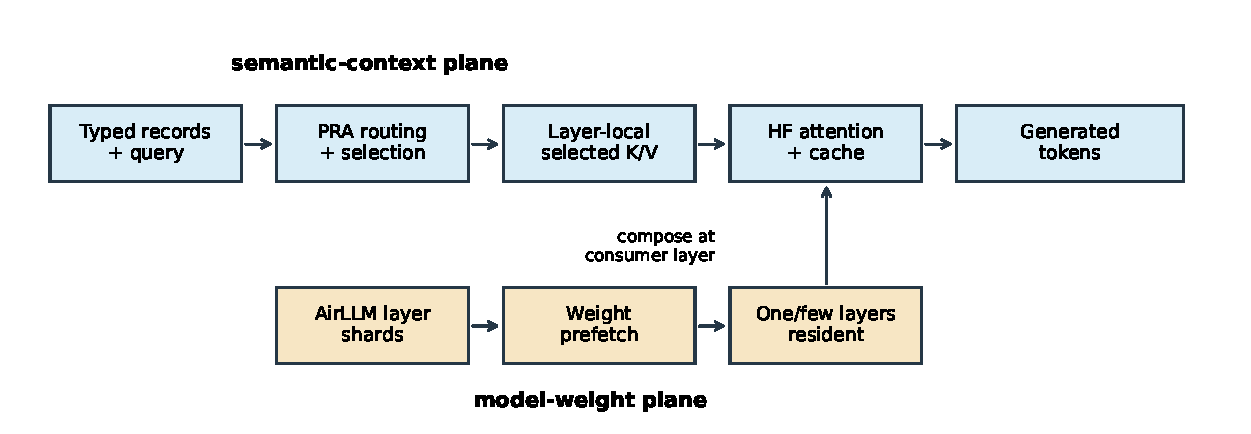
\includegraphics[width=\linewidth]{figures/airllm_pra_architecture.pdf}
  \caption{AirLLM owns weight-shard movement. The shared PRA runtime owns record
  identity, routing, authorization, and selected K/V. Their physical lifecycles
  compose at an HF attention consumer without sharing semantic policy.}
  \label{fig:architecture}
\end{figure}

We account for peak memory as
\begin{equation}
M_{\mathrm{peak}} = M_{\mathrm{weights,hot}} + M_{\mathrm{localKV}}
 + M_{\mathrm{PRA,hot}} + M_{\mathrm{temporary}} + M_{\mathrm{framework}}.
\end{equation}
PRA WARM/COLD bytes are reported separately because they are retained physical
state but not accelerator working-set bytes. This decomposition matters: once
AirLLM removes full-model residency, local K/V may become the dominant term.

\section{AirLLM Audit}

We pin AirLLM 3.3.0 at commit
\texttt{309999931a3cc5572d8880e7e0f18d408f3a067b}. The audit script records
source files and line numbers rather than inferring behavior from package names.
Table~\ref{tab:audit} summarizes the resulting contract.

\begin{table}[t]
\centering
\caption{AirLLM mechanisms and PRA consequences at the pinned revision.}
\label{tab:audit}
\small
\begin{tabular}{p{0.25\linewidth}p{0.35\linewidth}p{0.29\linewidth}}
\toprule
Mechanism & Source-audited behavior & PRA consequence \\
\midrule
HF execution & \texttt{self.model.generate} and \texttt{self.model} own generation/forward & Reuse HF PRA on CUDA/Linux \\
Model skeleton & Built under Accelerate meta initialization & Request device cannot be inferred from embedding residency \\
Weight lifecycle & Module pre-hook loads; post-hook returns weights to meta & Attach PRA lifecycle after weight hook \\
Prefetch & One-worker thread executor & Shared scheduling can serialize two reads \\
Pinned host memory & Per-prefetched-layer bound & PRA pinning needs a separate explicit budget \\
Sparse experts & Routed expert pre/post hooks when topology permits & Expert and context selection remain independent \\
macOS path & Separate \texttt{AirLLMLlamaMlx} implementation & E0 only; do not claim HF-native PRA \\
\bottomrule
\end{tabular}
\end{table}

The source audit found HF delegation in \path{airllm_base.py}, lines 904--907;
streaming-hook installation in the same file, lines 763--764; and expert hooks
near line 834. The Mac
dispatcher enters a separate MLX class in \texttt{auto\_model.py:7} and does
not expose AirLLM's HF \texttt{.model}. Consequently, platform capability is
not uniform: the Mac run validates AirLLM weight streaming and E0 selected text,
not native PRA.

\section{Integration}

\subsection{Capability-Gated Provider}

The shared provider registry now includes \texttt{airllm}. It advertises E0 by
default. Setting \texttt{native\_hf\_pra=true} enables E2 only on the
HF-backed path. The \texttt{storage\_managed} option changes how E2 tensors are
retained; it does not promote the path to E3 because AirLLM does not own their
complete scheduler lifecycle. The provider is embedded-only because AirLLM is
a Python model wrapper rather than an HTTP scheduler. This prevents the CLI and
product matrix from presenting the MLX path as native merely because the
package imports.

\subsection{Reusing HF Attention}

PRA wraps selected \texttt{self\_attn} modules while retaining each original
attention module as \texttt{original\_attention}. AirLLM shards still contain
ordinary keys such as
\begin{verbatim}
model.layers.7.self_attn.q_proj.weight
\end{verbatim}
The adapter maps that key, only for PRA-injected layers, to
\begin{verbatim}
model.layers.7.self_attn.original_attention.q_proj.weight
\end{verbatim}
at placement time. Checkpoint files are neither rewritten nor duplicated.
Unselected attention and all non-attention keys are unchanged. The request
device is taken from AirLLM's \texttt{running\_device}; relying on an embedding
parameter would incorrectly return \texttt{meta} when embeddings are streamed.

In simplified form, the native bridge is:
\begin{verbatim}
pra = PRAForCausalLM.from_model(airllm.model, airllm.tokenizer)
for shard_key, tensor in layer_shard:
    target = insert_original_attention(shard_key) if pra_layer else shard_key
    airllm.place(target, tensor)
pra.request_device = airllm.running_device
\end{verbatim}
AirLLM continues to invoke Transformers. PRA continues to use the model's own
Q/K/V projections, RoPE implementation, and cache semantics.

\subsection{Layer-Local PRA Lifecycle}

The lifecycle adapter registers its hooks after AirLLM. PyTorch therefore runs:
\begin{verbatim}
AirLLM pre: load W_l
PRA pre:    activate selected (K_l, V_l)
forward:    local attention + selected-memory attention
AirLLM post: release W_l
PRA post:   release (K_l, V_l), unless policy keeps it HOT
\end{verbatim}
The adapter supports three residency modes: HOT keeps every selected consumer
layer resident; \texttt{layer\_streamed} retains only the active layer;
\texttt{hybrid} keeps an explicit layer subset HOT. Closing an adapter releases
all active detail, enforcing the invariant that a later request cannot inherit
another request's selected memory.

\section{Experimental Method}

\subsection{Evidence Tiers}

\begin{itemize}
\item \evidence{Source audit}: pinned source and runtime-import facts.
\item \evidence{Live engine E0}: actual AirLLM/MLX model loading and generation.
\item \evidence{Controlled model}: measured hooks, stores, transfers, and memory
accounting with a deterministic eight-layer execution model; no language quality.
\item \evidence{Live native smoke}: CUDA HF-backed mechanism and parity tests.
\end{itemize}

\subsection{Live Apple Run}

The live E0 run used an Apple M5 with 16 GB unified memory, Python 3.11,
AirLLM 3.3.0, MLX 0.32.2, Transformers 5.12.1, and
\texttt{TinyLlama/TinyLlama-1.1B-Chat-v1.0}. AirLLM produced 50 shard/marker
files totaling 2,200,159,150 bytes. We froze one evidence sentence and compared
it as selected text against prompts containing repeated irrelevant archive notes.
Greedy decode emitted 12 tokens.

\subsection{Controlled Lifecycle Sweep}

The controlled model has eight decoder layers, four K/V heads, 64-dimensional
heads, FP16 K/V, 128 selected tokens, and 128 local query tokens. Each streamed
weight layer is modeled as 8 MiB over an 800-MiB/s store with 3 ms of layer
compute. We crossed backing contexts of 2K, 8K, 32K, and 64K tokens; three
consumer profiles; three residency modes; and three prefetch policies, then
added WARM, COLD, and SOURCE restoration controls. The result contains 119 rows
with three repeats for timed native conditions.

\section{Results}

\subsection{Selected Text on AirLLM/MLX}

\begin{table}[t]
\centering
\caption{Live AirLLM/MLX E0 generation. One run per condition; 12 greedy output
tokens. TTFT is first yielded token, not HTTP serving TTFT.}
\label{tab:mlx}
\small
\begin{tabular}{lrrrrl}
\toprule
Condition & Input tok. & TTFT (s) & Total (s) & tok/s & Output prefix \\
\midrule
Full, short & 185 & 7.65 & 89.18 & 0.135 & \texttt{The project access code is CYAN-ORBIT-} \\
Selected & 38 & 7.60 & 93.00 & 0.129 & same \\
Full, longer & 653 & 8.27 & 90.23 & 0.133 & same \\
Selected & 38 & 7.99 & 88.97 & 0.135 & same \\
\bottomrule
\end{tabular}
\end{table}

Selected text reduced visible input by 79.5\% relative to the 185-token prompt
and by 94.2\% relative to the 653-token prompt. It preserved the complete
12-token output prefix in all four conditions. The run stopped one generated
token before the final digits of the synthetic code, so we report prefix
agreement rather than exact-answer accuracy. Cold initialization, including
download/sharding, took 109.6 s; reuse of existing shards initialized in 0.57 s.
The first instrumented run observed about 1.10 GiB maximum change in system
available memory, while process RSS grew from 346 to 832 MiB. System-available
memory is noisy on a shared host and is not treated as process peak memory.

The small TTFT and throughput differences are the main result, not a failure of
selection. Each decoded token streams the model layers again. At these prompt
lengths, reducing sequential context cannot remove that fixed weight-I/O floor.
This finding motivates native persistent K/V chiefly for repeated queries and
longer backing contexts, not as a universal latency improvement.

The same run also exposed an AirLLM/MLX compatibility boundary: SmolLM2-135M
uses tied embeddings and had no independent \texttt{lm\_head} shard, but the
MLX generation path attempted to load one. We retain this blocked run as an
engine/model-family finding and do not count it as PRA evidence.

\subsection{HF-Backed CUDA Correctness}

\begin{table}[t]
\centering
\caption{Live AirLLM/HF execution on a 4-GiB GTX 950M. Four greedy output
tokens; peak is PyTorch CUDA allocation, not total device use.}
\label{tab:cuda}
\small
\begin{tabular}{lrrrr}
\toprule
Condition & Visible tok. & Native tok. & Total (s) & Peak (MiB) \\
\midrule
Full-context E0 & 377 & 0 & 40.29 & 160.42 \\
Selected-text E0 & 38 & 0 & 28.95 & 135.20 \\
PRA injected, disabled & 38 & 0 & 31.35 & 135.20 \\
Native PRA & 19 & 15 & 32.03 & 135.63 \\
\bottomrule
\end{tabular}
\end{table}

The full and selected E0 conditions generated the same four-token prefix.
Selected text removed 89.9\% of visible input, reduced completion latency by
28.2\%, and reduced peak allocated CUDA memory by 15.7\%. After PRA injection,
the disabled condition matched the selected E0 token sequence exactly. This is
the key parameter-placement result: every streamed decoder shard reached the
PRA-wrapped path without changing disabled semantics.

Reference encoding took 7.12 s for 15 tokens. Native generation exposed only
19 query tokens sequentially and materialized all 15 selected K/V tokens at the
configured final four consumer layers. It generated the same prefix in 32.03 s
and peaked at 135.63 MiB. Relative to selected-text E0, this is a 10.6\% latency
cost and 0.3\% peak-allocation increase in a cold one-query smoke. Persistent
reuse is therefore the economic gate: the one-time 7.12-s encoding cost must be
amortized across repeated queries before native PRA can improve this frontier.

\subsection{Selector-Frozen Natural Follow-Up}

We next froze one routed selection from each of QASPER, HotpotQA, and
2WikiMultiHopQA. Selected-text E0 and native E2 received the same evidence;
E2 consumed 384 selected native tokens through the final four layers. Each
condition used one cold generation and two warm repetitions. Table
\ref{tab:cuda-natural} is generated from the raw JSON artifact.

\begin{table}[t]
\centering
\caption{Natural AirLLM/HF follow-up on the GTX 950M. Time is completion time;
lower E2/E0 is better. Pair exact compares complete E0 and E2 output strings.}
\label{tab:cuda-natural}
\small
\begin{tabular}{llrrrrr}
\toprule
Dataset & State & E0 F1 & E2 F1 & Pair exact & E2/E0 time & Visible $\downarrow$ \\
\midrule
2Wiki & cold & 0.000 & 0.000 & 0.000 & 1.003 & 93.5\% \\
2Wiki & warm & 0.000 & 0.000 & 0.000 & 0.969 & 93.5\% \\
HotpotQA & cold & 0.000 & 0.000 & 0.000 & 0.991 & 92.9\% \\
HotpotQA & warm & 0.000 & 0.000 & 0.000 & 1.013 & 92.9\% \\
QASPER & cold & 0.000 & 0.000 & 0.000 & 1.016 & 95.8\% \\
QASPER & warm & 0.000 & 0.000 & 0.000 & 1.005 & 95.8\% \\
\bottomrule
\end{tabular}

\end{table}

Native execution removed 92.9--95.8\% of the visible selected-text prompt and
reduced peak allocated CUDA memory from 171--175 MiB to 136--137 MiB. Its
completion time stayed close to E0: the six cold/warm ratios span
0.969--1.016. Reference encoding, however, averaged 19.26 s and must be
amortized separately. These are positive bounded-context and residency results.

They are not a quality result. TinyLlama scored zero token F1 in both
representations on all three examples, and E2 matched none of nine E0 output
strings. The partial four-layer native consumer is not execution-equivalent to
placing the same evidence in every ordinary decoder layer. A larger cohort with
a capable model and a full-consumer reference is required before promoting
native E2 beyond research-only status.

\subsection{Residency Frontier}

\begin{figure}[t]
  \centering
  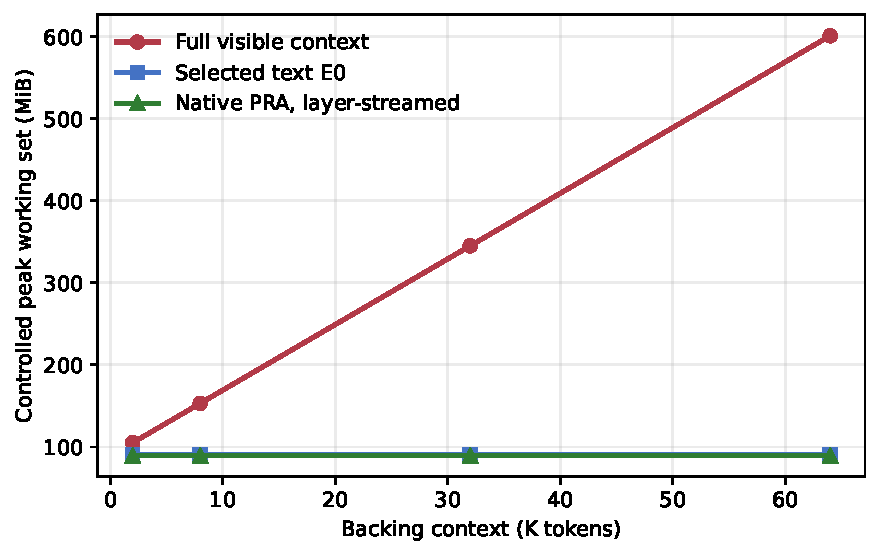
\includegraphics[width=0.78\linewidth]{figures/context_memory_frontier.pdf}
  \caption{Controlled working-set decomposition. Full-context local K/V grows
  with backing length; selected text and native selected K/V remain bounded.
  These values are model-derived accounting, not GPU telemetry.}
  \label{fig:memory}
\end{figure}

At 32K backing tokens under the balanced four-consumer profile, HOT PRA retained
0.50 MiB, hybrid retained 0.375 MiB, and layer-streamed PRA retained 0.125 MiB.
Thus layer streaming reduced peak PRA detail by 4$\times$ relative to HOT for
the same 128 selected tokens. In the controlled decomposition at 64K,
full-context execution reached 601.0 MiB while balanced layer-streamed native
PRA reached 89.125 MiB. The 85.2\% reduction follows directly from holding
selected evidence and query length fixed; it is a memory-accounting result, not
evidence that 64K model quality is preserved.

\subsection{Prefetch Interaction}

\begin{figure}[t]
  \centering
  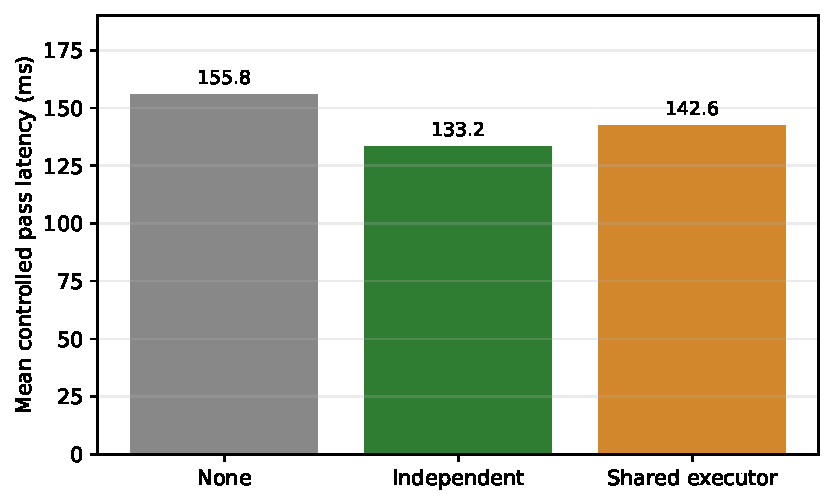
\includegraphics[width=0.68\linewidth]{figures/prefetch_overlap.pdf}
  \caption{Controlled 32K/hybrid balanced-profile latency. Sharing AirLLM's
  one-worker executor avoids another thread but queues PRA behind weight reads.}
  \label{fig:prefetch}
\end{figure}

For the 32K balanced hybrid condition, no PRA prefetch took 155.83 ms per
controlled pass. Independent one-worker PRA prefetch took 133.25 ms, a 14.5\%
reduction. Coordinated prefetch on AirLLM's weight executor took 142.56 ms, 8.5\%
below no prefetch but 7.0\% above independent prefetch. ``Coordinated'' is
therefore not synonymous with ``faster'': a shared serial queue can prevent
thread multiplication yet lose useful overlap. A production controller should
choose between independent I/O and queue coordination from observed storage
parallelism rather than platform labels.

\begin{table}[t]
\centering
\caption{Evidence status at this revision.}
\label{tab:status}
\small
\begin{tabular}{p{0.34\linewidth}p{0.18\linewidth}p{0.37\linewidth}}
\toprule
Claim & Status & Evidence boundary \\
\midrule
AirLLM delegates CUDA forward/generate to HF & Established & Pinned source audit \\
AirLLM/MLX runs layer-streamed TinyLlama & Established & Live M5 E0 run \\
Selected text preserves tested answer prefix & Established & Four live conditions, one example \\
PRA K/V can follow a layer-local lifecycle & Established & Tests plus 119-row controlled sweep \\
Native HF parameter placement bridge & Established & Unit tests and live disabled parity \\
Native AirLLM/PRA mechanism & Established & Live CUDA smoke plus three natural examples \\
Natural E0/E2 semantic parity & Open & 0/9 exact pairs; task F1 uninformative at zero \\
Large-model-beyond-VRAM advantage & Open & Requires a model larger than accelerator memory \\
\bottomrule
\end{tabular}
\end{table}

\section{What the Results Do and Do Not Establish}

The measurements establish a clean ownership boundary and a feasible physical
lifecycle. They show that a bounded selected context does not inherit backing
context's K/V growth in the accounting model. They also show that AirLLM's
weight-streaming cost can dominate short-prompt E0 inference, and that using one
executor for two I/O streams may be inferior to bounded independent prefetch.

They do not establish that native PRA improves answer quality or TTFT for a
model that cannot fit on the test accelerator. The natural follow-up does show
lower allocated CUDA peak and near-parity completion time, but the three-example
cohort has zero task F1 and divergent E0/E2 sequences. The small CUDA smoke
closes AirLLM disabled, injected-but-disabled, reference encoding, and native
consumption. A scale claim still requires a conventional HF baseline, repeated
decode, HOT versus layer-streamed native PRA, matched source/query geometry, and
frozen selected intervals on a larger natural cohort.

\section{Product Contract}

The current product row is deliberately conservative:
\begin{center}
\small
\begin{tabular}{lllll}
\toprule
Engine & Platform & Default & Native candidate & Evidence tier \\
\midrule
AirLLM & macOS/MLX & E0 selected text & unavailable & live smoke \\
AirLLM & CUDA/HF & E0 selected text & opt-in E2 & natural transport candidate \\
\bottomrule
\end{tabular}
\end{center}
The runtime exposes \texttt{airllm} only as an embedded provider. Native flags
must be explicit. No \texttt{QUALITY\_MAX} product claim follows from this
small calibration; profiles remain candidates until natural-task validation.

\section{Limitations and Next Experiments}

The M5 cohort is one synthetic retrieval example and one Llama-family model.
Its MLX path differs architecturally from AirLLM's HF path. The controlled model
uses explicit bandwidth and compute parameters and cannot estimate kernel-level
attention cost or language quality. The host was under unrelated memory load,
so available-memory deltas are supporting diagnostics only.

The next decisive experiment is not another hook microbenchmark. On a newer
CUDA host, repeat the frozen-selection comparison with a capable model, at
least 50 examples per dataset, and both full-consumer and economical
late-consumer E2. Extend it to multi-query same-resource and shared-resource
reuse. Report answer F1/EM, gold log probability, visible and native tokens,
weight and PRA bytes, TTFT, inter-token latency, peak memory decomposition, and
cache hits. Then repeat on a model materially larger than VRAM. A sparse-MoE run
is useful only after dense-model correctness; expert selection and PRA routing
must remain separately attributed.

\section{Related Work}

AirLLM~\cite{airllm} belongs to layer/expert streaming and offload systems.
FlexGen~\cite{flexgen} jointly schedules parameters, activations, and K/V across
GPU, CPU, and disk for throughput-oriented constrained inference. Transformers
provides the architecture and cache semantics reused by the integration
described here~\cite{transformers}. PagedAttention and vLLM~\cite{vllm} address
fragmentation and sharing of sequential serving K/V; their scheduler-visible
block abstraction differs from AirLLM's layer-streamed parameter lifecycle.
Retrieval and prompt compression move selected text into the ordinary prefix.
PRA instead studies query-selected non-prefix native state. The distinguishing
combination here is parameter streaming plus semantic K/V selection, with the
two policies remaining independently measurable.

\section{Conclusion}

AirLLM and PRA target different memory terms and can share an HF execution path
without sharing policy. The integration requires more than calling two APIs:
PRA-wrapped parameter names must be reconciled with AirLLM shards, request
device identity cannot be read from meta-resident embeddings, teardown must
prevent selected-detail leakage, and prefetch queues must be measured rather
than assumed. Live MLX E0 results show substantial visible-token reduction but
also expose weight streaming as the dominant latency floor. Controlled results
show a 4$\times$ PRA peak-residency reduction from layer-local streaming and a
prefetch tradeoff between independent overlap and shared-queue discipline. A
live CUDA smoke closes parameter-placement, disabled-parity, reference-encoding,
and native-consumption gates. The natural follow-up removes 92.9--95.8\% of
visible selected-text tokens at near-parity completion time and lower allocated
CUDA peak, but its zero task F1 and 0/9 exact output pairs leave semantic parity
open. The remaining scientific gate is adequately powered natural quality at a
scale where both weight and context virtualization are necessary.

\section*{Reproducibility}

Scripts are in \texttt{experiments/paper6\_6\_airllm}. Raw JSON, figures, and
the source capability audit are under
\texttt{docs/papers/shared/results/paper6\_6\_airllm} and the paper's
\texttt{figures} directory. Unit tests cover provider negotiation, selective
parameter-key remapping, lifecycle ordering, HOT reuse, teardown, and memory
decomposition. Every live artifact records package versions, hardware, model,
and its evidence tier.

\begin{thebibliography}{9}
\small
\bibitem{airllm}
G. Lyongavin et al. \emph{AirLLM: Run large language models on low-end GPUs}.
Pinned source repository, 2026. \url{https://github.com/lyogavin/airllm}.

\bibitem{transformers}
T. Wolf et al. Transformers: State-of-the-art natural language processing.
\emph{EMNLP: System Demonstrations}, 2020.

\bibitem{flexgen}
Y. Sheng et al. FlexGen: High-throughput generative inference of large language
models with a single GPU. \emph{ICML}, 2023.

\bibitem{vllm}
W. Kwon et al. Efficient memory management for large language model serving
with PagedAttention. \emph{SOSP}, 2023.
\end{thebibliography}

\end{document}
